\section{The defense}\label{sec:defense}
Keeping in mind our theoretical model, we determine the key elements that make these
attacks possible.

We propose a defense, \textit{context hiding}, that mitigates a class of
practical compression side-channel attacks such as CRIME, TIME, BREACH, Rupture,
and HEIST. The full plaintext recovery these attacks perform is no longer
possible when our defense is applied.

\subsection{Hardness of defending}
First of all, observe that there is a trivial method of defense, and that is
disabling compression completely.

However, defending against an adversary by modifying $f$ is hard in general. We
note that $f$ is required to be polynomially reversible, meaning it must contain
enough information to recover $s$. Because $Com$ must be able to decrease the
length of various plaintexts, it can output plaintexts of different lengths
dependent on $s$. Therefore, if $Com$ is adversarial, it can easily leak
information through the encryption function $Enc$ by using its output length. As
such, any attempt to generally defend against all compression functions $Com$ is
necessarily futile.

However, the fact that it is theoretically difficult to define a generic defense
should not discourage us from pursuing a practical defense that applies in
practice given the specific compression functions currently in use in the
real-world.  In this direction, we give a series of arguments for why we believe
our defense method is secure based on our previously developed theory.

\subsection{Attack elements from a defense perspective}
The basic problem that needs be solved is the compression detectability of the
predicate $Q$ under this class of attacks. In order to eliminate detectability,
it should be made impossible for any pair of reflections $\overbar{r}$ to detect
$Q$ under the compression function $\textrm{Com}$ and the rendering function
$f$. In order to achieve this there exist two options - either change the
compression or the rendering function.

The next step is determining what what kind of changes are needed. We therefore
consider the notions that make detectability possible. These notions are
compression idealness and interdependence. The first is part of the composition
of $\textrm{Com}$ and $f$ whereas the second is part of $f$. That said, removing
either of these notions from the functions will strip the adversary the ability
to detect $Q$.

The first choice is forcing the compression function to act non-ideally in the
cases of secrets. Proposed defenses like disabling compression for annotated
secrets incorporate this exact idea.

The second choice is removing the interdependece between reflections and
secrets. In order to achieve that we need to decorrelate the probability of
secrets and reflections. A method that acts similarly is secret masking,
described in section \ref{subsec:masking}. Context hiding also builds on this
option and is described in the following sections.

\subsection{Context hiding properties}

Context hiding is built on the premise of separating secrets in a per-origin
manner in order to avoid cross-compression. In order to achieve this we define
what constitutes an origin and what properties same-origin secrets share.

\subsubsection{Origins}
An origin is a uniquely identifiable party that generates content. A party can
be either a physical entity, like a user, or an application. It is important to
properly identify the party that generated a piece of content, as the definition
of origins reflects the amount of knowledge on same-origin content.

\subsubsection{Same-origin secrets}
After defining the origins, we separate the secrets as content pieces assigned
to origins. All secrets assigned to an origin should have been generated by the
party that this origin identifies. An immediate result of this definition is
that anyone with access to a secret $s$ of origin $o$ also has access to all
other secrets $s'$ of the same origin $o$.

\subsection{Context hiding functionality}
Our defense method disables cross-compression by applying a simple substitution
cipher derived from a random permutation of the plaintext alphabet.

Firstly, we identify the origins of the plaintext $m$ and store them in the
array $origins$. Each secret $s_i$ in $m$ is identified by its origin. Each
origin is uniquely identified by an integer in range $[0, |origins|-1)$.

Secondly, we identify the alphabet for each origin. An origin's alphabet is the
set of characters of all secrets in this origin. For each origin, we generate a
random permutation of the origin's alphabet and store it in the array
$permutations$. The first element in the $permutations$ array corresponds to the
first origin in the $origins$ array and so forth.

In order to secure the secret $s$ we apply a hiding function. This function
\textit{hide} takes two arguments, the secret $s$ and the permutation $p$ of the
secret's origin. It applies the substitution cipher on each character in $s$ and
returns the permuted secret $s'$. The substitution cipher is implemented in the
function $Permute_p(c)$, which returns the $i$-th character in $p$, $i$ being
the index of $c$ in the clear alphabet.

\begin{lstlisting}[texcl,mathescape,basicstyle=\small]
def hide($s, p$):
    $s' = ''$
    for $ch \in s$:
        $s' = s' || Permute_p(ch)$
    return $s'$
\end{lstlisting}

The protected secret $s'$ is annotated by the special characters
$\beta_{start}^i$, $\beta_{end}^i$ that mark the start and the end of any
substring that needs to be unpermuted and are unique per origin. The output $m'$
that is produced after hiding all secrets consists of all permuted texts
concatenated with the permutation array $permutations$.

The initial secret $s$ can be retrieved from the protected secret $s'$ using the
\textit{unhide} function. This function takes $s'$ and permutation $p$ of the
secret's origin, applies the reverse permutation on $s'$, and returns the
unpermuted secret $s$.

\begin{lstlisting}[texcl,mathescape,basicstyle=\small]
def unhide($s', p$):
    $s = ''$
    for $ch \in s'$:
        $s = s || Permute_p^{-1}(ch)$
    return $s$
\end{lstlisting}

In our theoretical model, we assume that there exists a single secret. However,
in this section we generalize this and, in practice, the reflection $r$ and the
secret $s$ are handled as two secrets that have different origins. The fact
that $s$ and $r$ are permuted every time an oracle call is made makes it
impossible for an adversary controlling $r$ to learn information about $s$.

Our defense is implemented in the application layer and is opt-in. We choose to
update the rendering function $f$ instead of the compression function
$\textrm{Com}$ as it is easier for web developers to incorporate it in their
applications. Our proposal requires no changes in the underlying compression
algorithms in the web server such as Apache's mod\_deflate, which would require
a huge engineering effort. Instead, it only requires modifications in the web
application layer and can be relatively easily incorporated in existing
applications.

\section{CTX: Mitigating BREACH with Context Hiding }\label{sec:ctx}

\subsection{Implementation}
Our contributions include the development of the CTX defense. CTX is an
implementation of the context hiding method described in the previous section
for HTML web pages.

It is up to the application developer to decide which portions of the response
are sensitive and must be protected as secrets. Sensitive data does not only
include high-value secrets such as passwords and CSRF tokens, but also any data
that the developer wishes to keep private. Some examples are the bodies of email
messages, chat messages, or the contents of documents and spreadsheets, as they
contain all the important contacts of the victim. Practically any piece of
information which is only accessible when logged in is a secret and should be
CTX protected. On the other hand, some data do not typically need
compression-security protection, e.g. static HTML portions that are accessible
on a website even when logged out.

The minimum amount of origins is one origin for the entire response, in which
case CTX is not protecting any part of the plaintext, and the maximum is one
origin per character. The latter would result in the best possible security
under CTX, although compression would be effectively disabled. This is the case
with defenses such as secret masking.

Different-origin secrets are then forced to compress separately, i.e. not
cross-compress. However, compression is achieved within each context. The
default origin alphabet is ASCII characters (0 - 128). In order to randomly
permute the secret alphabet, we use the Fisher-Yates shuffle
algorithm \cite{fisher1938statistical}.

Secrets are then permuted by the server using the generated permutation of the
secret's origin, encrypted by TLS, and sent over the network. Upon arrival on
the client side, the inverse permutation is applied to decode the secret.

Each time the server issues an HTTPS response, new per-origin permutations are
generated. Compression side-channel attacks in general rely on the assumption
that we can perform multiple requests to the target website while the
transmitted secret remains the same. Since new alphabet permutations are
generated per HTTPS response, the statistical analysis performed by Rupture is
no longer feasible.

\subsection{Experimental results}\label{subsec:ctx_experiments}

We have conducted several experiments to evaluate the performance of web
services protected by CTX. The results of these experiments are overwhelmingly
positive.

The CTX parameters that affect performance are basically 3: the number of
origins, the total response size in bytes, and the amount of
secrets in the response. Each parameter affects the performance differently and
will be examined thoroughly in the following sections. Our experiments focused
on each parameter separately, so the results reflect the performace under each
one independently.

In all our tests we use an HTML web page where the secrets are strings of
English literature. The tests measure the performance penalty in terms of size
overhead in the compressed response HTML. The penalty in execution time is
considered insignificant and not included when less than 10ms.

However, it should be noted that our tests are particularly strict. A typical
website response consists mainly of HTML code or libraries that usually need not
be protected. In this case, the amount of secrets in the response would not
exceed 1\% of the total response, in which case the CTX overhead as shown by our
experiments is acceptable. For example, Facebook and Gmail, which offer web
pages that are ~600KB typically need only protect approximately 0.5\% of the
response.

The first parameter, the number of origins, mainly affects the compression
performance of the secrets. The more origins are used the bigger the response,
both compressed and uncompressed, will be. This is expected, given the fact that
secrets from different origins do not cross-compress.

Our experiment covered a 650KB web page, which consists of 1\% secrets and 99\%
static data. The secrets are distributed in origins that range from 1 to 50, so
the length of a secret per origin is reduced as origins increase and the total
amount of secrets and static data remains the same. We consider 50 origins a
reasonable choice since a typical response contains data generated by multiple
users and web services.

    \begin{figure}[thpb]
        \centering
            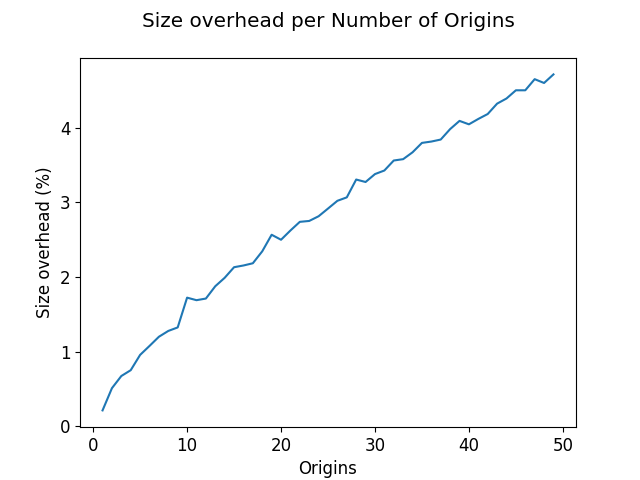
\includegraphics[width=0.48\textwidth]{experiments/origins.png}
        \caption{Origins}
        \label{fig:origin_ctx}
    \end{figure}

As Figure \ref{fig:origin_ctx} shows, the size overhead when 1 origin is used is less than 0.5\%
and about 4.7\% when 50 origins are used. This means that the compressed
response when CTX is used is expected to be 1.47x the unprotected compressed
response when 50 origins are used.

The second parameter, the total response size in bytes, affects the impact of
CTX on the compressed response.

In this case, we use 50 origins and consider 1\% of the total response to be
secret, equally distributed in all origins. The total response ranges from a
13KB to a 650KB web page.

Our experiments show that the increase in bytes that CTX adds is not
proportional to the increase of the total response size. This results in a
significant response size increase for small web pages, which becomes less
observable as the web page grows larger.

    \begin{figure}[thpb]
        \centering
            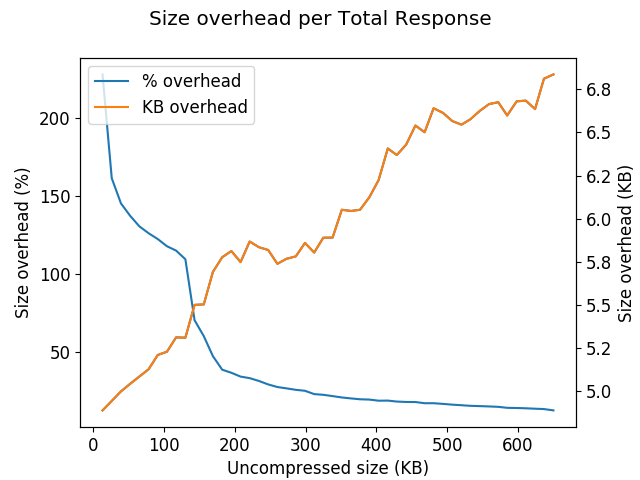
\includegraphics[width=0.48\textwidth]{experiments/total_response.png}
        \caption{Total response}
        \label{fig:total_response_ctx}
    \end{figure}

Figure \ref{fig:total_response_ctx} depicts the results of this experiment. A 13KB web page suffers a 5KB
CTX overhead, which corresponds to a 228\% increase in compressed response. On the
other hand, CTX will add only 7KB of compressed data for a 650KB web page, which
results in a 12\% increase. Disabling compression entirely would add overhead
that ranges from 500\% to 1000\% for the tested web pages.

The third parameter is the total amount of secrets in the response. In our
example we use a 650KB web page with 50 CTX origins. The secrets range from 1\%
up to 50\% of the web page, the rest being static data, and are evenly
distributed across origins.

    \begin{figure}[thpb]
        \centering
            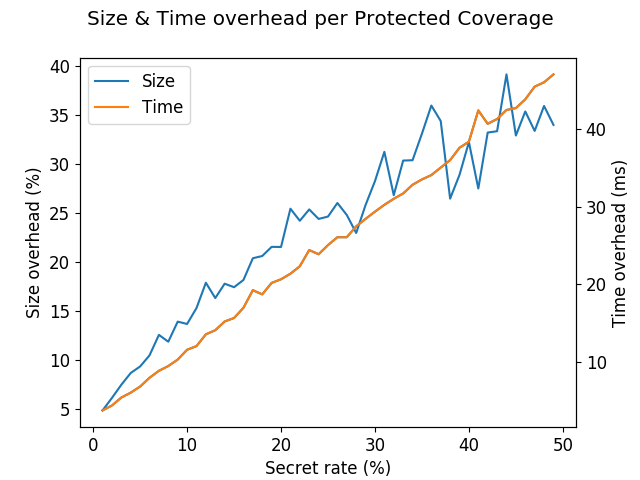
\includegraphics[width=0.48\textwidth]{experiments/response_secrets.png}
        \caption{Response secrets}
        \label{fig:response_secrets_ctx}
    \end{figure}

Figure \ref{fig:response_secrets_ctx} shows the results in this case. We find that protecting 1\% of the
tested web page results in less than 5\% size overhead, whereas protecting 50\% of
the page results in 35\%. This test also showed a noteworthy time increase in
execution time, where for 10\% secrets in the web page CTX adds 10ms of
execution time, while for 50\% it adds 47ms.

In comparison, disabling compression would again result in 976.8\% load overhead
and a network transmittion time overhead that, depending on the client's and the
server's network, may be several seconds.


In order to back our claim, we perform the following experiment. We choose a
fixed secret $s$, 100 characters long. We then choose the reflections $r_i,
i\in[0, 50]$, where $|r_i| = 50 + i*20$. For each $r_i$ we calculate the
length of separate compression using gzip $|gzip(s)||gzip(r_i)|$ and the length
of the compressed CTX'ed secret and reflection $|gzip(ctx(s), ctx(r_i))|$, where $s$
and $r_i$ belong to different origins.

The results are shown in figure \ref{fig:defense_experiment}. It can be seen
that the outputs of these two methods are linearly correlated, while also the
Pearson correlation coefficient of the two variables is 0.998712.

    \begin{figure}[thpb]
        \centering
            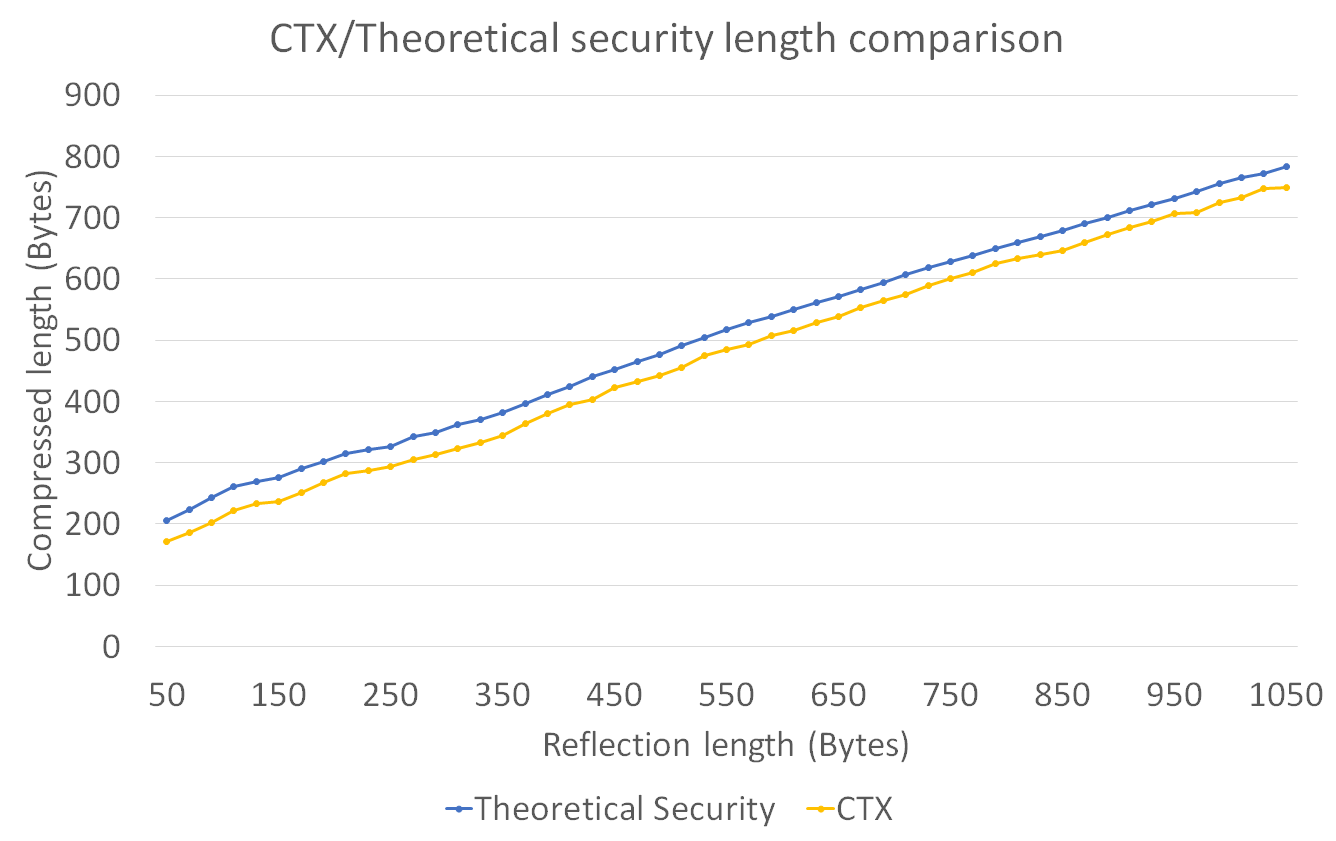
\includegraphics[width=0.48\textwidth]{defense_experiments/ctx_experiment.png}
        \caption{CTX/Theoretical security comparison}
        \label{fig:defense_experiment}
    \end{figure}
